\begin{figure}[t]
\centering
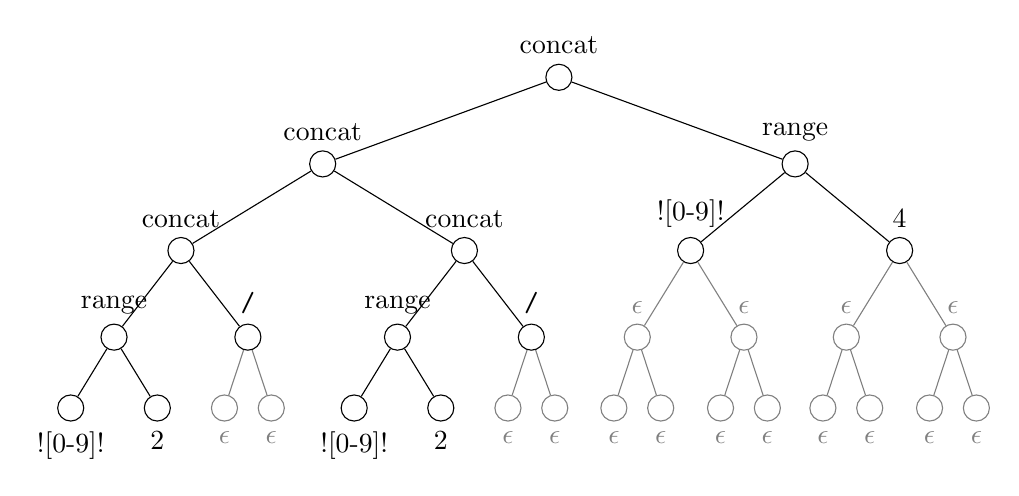
\begin{tikzpicture}[
level distance=1.1cm,
level 1/.style={sibling distance=6cm},
level 2/.style={sibling distance=3.6cm},
level 3/.style={sibling distance=1.7cm},
level 4/.style={sibling distance=1.1cm,level distance=.9cm}]
\tikzstyle{every node}=[circle,draw,minimum size=1.4pt]
\tikzstyle{every label}=[rectangle, draw=none]

\node (Root) [label={concat}] {}
child {
    node [label={concat}] {} 
    child {
        node [label={concat}] {} 
        child {
            node [label={range}] {} 
            child { node [label=below:{\Verb![0-9]!}] {} }
            child { node [label=below:{2}] {} }
        }
        child {
            node [label={\texttt{/}}] {} 
            child { node [label={[text=gray]below:\(\epsilon\)}, draw=gray, right=.08cm] {} edge from parent[draw=gray] }
            child { node [label={[text=gray]below:\(\epsilon\)}, draw=gray, left=.08cm] {} edge from parent[draw=gray] }
        }
    }
    child {
        node [label={concat}] {} 
        child {
            node [label={range}] {} 
            child { node [label=below:{\Verb![0-9]!}] {} }
            child { node [label=below:{2}] {} }
        }
        child {
            node [label={\texttt{/}}] {} 
            child { node [label={[text=gray]below:\(\epsilon\)}, draw=gray, right=.08cm] {} edge from parent[draw=gray] }
            child { node [label={[text=gray]below:\(\epsilon\)}, draw=gray, left=.08cm] {} edge from parent[draw=gray] }
        }
    }
}
%
child {
    node [label={range}] {} 
    child {
        node [label={\Verb![0-9]!}, right=.3cm] {}
        child {
            node [label={[text=gray]:\(\epsilon\)}, draw=gray, right=0cm] {} edge from parent[draw=gray]
            child { node [label={[text=gray]below:\(\epsilon\)}, draw=gray, right=.08cm] {} edge from parent[draw=gray] }
            child { node [label={[text=gray]below:\(\epsilon\)}, draw=gray, left=.08cm] {} edge from parent[draw=gray] }
        }
        child {
            node [label={[text=gray]:\(\epsilon\)}, draw=gray, left=0cm] {} edge from parent[draw=gray]
            child { node [label={[text=gray]below:\(\epsilon\)}, draw=gray, right=.08cm] {} edge from parent[draw=gray] }
            child { node [label={[text=gray]below:\(\epsilon\)}, draw=gray, left=.08cm] {} edge from parent[draw=gray] }
        }
    }
    child {
        node [label={4}, left=.3cm] {}
        child {
            node [label={[text=gray]:\(\epsilon\)}, draw=gray, right=0cm] {} edge from parent[draw=gray]
            child { node [label={[text=gray]below:\(\epsilon\)}, draw=gray, right=.08cm] {} edge from parent[draw=gray] }
            child { node [label={[text=gray]below:\(\epsilon\)}, draw=gray, left=.08cm] {} edge from parent[draw=gray] }
        }
        child {
            node [label={[text=gray]:\(\epsilon\)}, draw=gray, left=0cm] {} edge from parent[draw=gray]
            child { node [label={[text=gray]below:\(\epsilon\)}, draw=gray, right=.08cm] {} edge from parent[draw=gray]}
            child { node [label={[text=gray]below:\(\epsilon\)}, draw=gray, left=.08cm] {} edge from parent[draw=gray]}
        }
    }
};

\end{tikzpicture}
\caption{\UseVerb{date2} represented as a \(k\)-tree.}
\label{fig:date-ktree}
\end{figure}{}